\documentclass[12pt]{article}

\usepackage[margin = .8in]{geometry}
\usepackage{amsmath}
\usepackage{graphicx}
\usepackage{multicol, enumerate, tabularx}
\usepackage{booktabs}
\usepackage{array}
\usepackage{adjustbox}

\usepackage{fancyhdr}
\pagestyle{fancy}

\lhead{Math F113X: Math and Society}
\rhead{Graph Theory}

\usepackage{tikz}
\usetikzlibrary{calc,trees,positioning,arrows,fit,shapes,through, backgrounds}
\usetikzlibrary{patterns}

\usetikzlibrary{decorations.markings}
\usetikzlibrary{arrows}

\usepackage{pgfplots}

\usepackage{longtable}
\usepackage{tabularx}

\newcommand{\ds}{\displaystyle}
\newcommand{\ans}[1][1in]{\rule{#1}{.5pt}}

\newcommand{\points}[1]{(#1 points.)}		% Trying to be lazy.

\usepackage{array}
\newcolumntype{L}[1]{>{\raggedright\let\newline\\\arraybackslash\hspace{0pt}}m{#1}}
\newcolumntype{C}[1]{>{\centering\let\newline\\\arraybackslash\hspace{0pt}}m{#1}}
\newcolumntype{R}[1]{>{\raggedleft\let\newline\\\arraybackslash\hspace{0pt}}m{#1}}
\newcommand{\red}[1]{\textcolor{red}{#1}}

\newcommand{\be}{\begin{enumerate}}
\newcommand{\ee}{\end{enumerate}}

%\topmargin -1in
%\textheight 9.5in
%\oddsidemargin -0.3in
%\evensidemargin \oddsidemargin
%\pagestyle{empty}
%%\marginparwidth 0.5in
%\textwidth 7in
%\parindent 0in

%--------------------------------------------------------------------------------------------------------------------------------------------------------------------------
%						Document
%--------------------------------------------------------------------------------------------------------------------------------------------------------------------------


% Partial Sorted Edges picture: #1 = chosen edges, #2 = candidate (dashed) edge
\newcommand{\partialSE}[2]{%
\begin{tikzpicture}[baseline=(current bounding box.center), scale=.8]
\tikzstyle{vtx}=[draw, circle, fill=white, inner sep =1.5 pt, font=\footnotesize]
\foreach \i/\l in {0/A,1/B,2/C,3/D,4/E}{\node[vtx] (\i) at (90+72*\i:1.2){\l};}
\begin{scope}[on background layer]
\foreach \i/\j in {#1}{\draw[line width=1.5pt] (\i) -- (\j);}
\foreach \i/\j in {#2}{\draw[dashed, thick] (\i) -- (\j);}
\end{scope}
\end{tikzpicture}}

\begin{document}
%\pagestyle{fancy}

\begin{center}
{\Large  Worksheet:  Hamiltonian Circuits \& Sorted Edges / Cheapest Link	}
\end{center}

\noindent \textbf{Group Names:} \hrulefill

\medskip

\noindent\fbox{\parbox{\dimexpr\linewidth-2\fboxsep-2\fboxrule}{\textbf{Sorted Edges / Cheapest Link:} Sort the edges from cheapest to most expensive. Add the next cheapest edge to your circuit \emph{unless}
(1) it closes the circuit too soon, or (2) it creates a degree 3 vertex.
Break ties by choosing the alphabetically smallest edge.}}

%-------------------------------------------------------------------------------------------------------------
%						Assignment
%-----------------------------------------------------------------------------------------------------
\begin{enumerate}

\item In each picture, the thick edges have already been chosen by the Sorted Edges algorithm, and the dashed edge is the next cheapest edge. Should the dashed edge be added? If not, which rule does it break?

\medskip

\begin{tabularx}{\linewidth}{X X X X}
(a) & (b) & (c) & (d) \\
\partialSE{0/1,1/2}{2/0} & \partialSE{0/1,0/2}{0/3} & \partialSE{0/1,2/3}{1/2} & \partialSE{0/1,1/2,2/3,3/4}{4/0}
%\\[10pt]
%\ans[.8in] & \ans[.8in] & \ans[.8in] & \ans[.8in] \\[16pt]
%\ans[.8in] & \ans[.8in] & \ans[.8in] & \ans[.8in]
\end{tabularx}

\vfill
\vfill

\item Apply the Sorted Edges algorithm to the graph below to find a Hamiltonian circuit. Draw in the edges, labeled with their weight, as you add them on the empty graph, and keep track of each step in the table. Break ties by choosing the alphabetically smaller edge.

\medskip

\begin{adjustbox}{valign=t,minipage={.4\textwidth}}
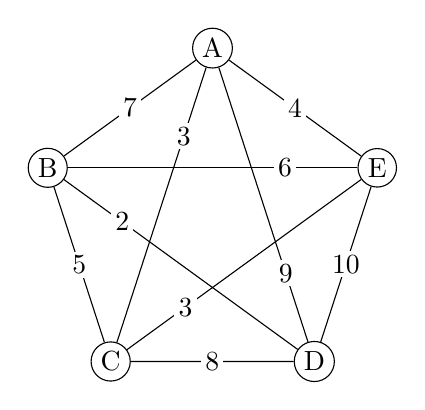
\begin{tikzpicture}[scale=1.1]
\tikzstyle{vtx}=[draw, circle, fill=white, inner sep =1.5 pt]
\tikzstyle{lbl}=[inner sep =1.5 pt, fill = white]
\foreach \i/\l in {0/A,1/B,2/C,3/D,4/E}{\node[vtx] (\l) at (90+72*\i:2){\l};}
\begin{scope}[on background layer]
\foreach \i/\j/\w in {A/B/7,B/C/5,C/D/8,D/E/10,E/A/4}{\draw (\i) -- node[lbl]{\w} (\j);}
\foreach \i/\j/\w in {A/C/3,D/A/9,B/D/2,E/B/6,C/E/3}{\draw (\i) -- node[lbl, pos=.25]{\w} (\j);}
\end{scope}
\end{tikzpicture}
\end{adjustbox}
\hfill
\begin{adjustbox}{valign=t,minipage={.4\textwidth}}
\begin{tikzpicture}[scale=1.1]
\tikzstyle{vtx}=[draw, circle, fill=white, inner sep =1.5 pt]
\foreach \i/\l in {0/A,1/B,2/C,3/D,4/E}{\node[vtx] (\l) at (90+72*\i:2){\l};}
\end{tikzpicture}
\end{adjustbox}

\bigskip

\begin{adjustbox}{valign=t,minipage={.5\linewidth}}
\begin{tabular}{ c | c | p{1.6in} }
Sorted edges & weight & used? (or why not) \\ \hline
$BD$ & 2 & \\ \hline
$AC$ & 3 & \\ \hline
$CE$ & 3 & \\ \hline
$AE$ & 4 & \\ \hline
$BC$ & 5 & \\ \hline
$BE$ & 6 & \\ \hline
$AB$ & 7 & \\ \hline
$CD$ & 8 & \\ \hline
$AD$ & 9 & \\ \hline
$DE$ & 10 & \\ \hline
\end{tabular}
\end{adjustbox}
\hfill
\begin{adjustbox}{valign=t,minipage={.42\linewidth}}
\raggedright
List the vertices of the Hamiltonian circuit, starting at vertex A.

\medskip
\hrulefill

\bigskip

Total weight of the circuit: \ans

\bigskip

%Why did you have to use a tie-breaking rule in this problem?
\end{adjustbox}

\vfill

\newpage

\item On the previous worksheet, you used Nearest Neighbor to plan a tour of the six most populous cities in Africa. Here is the same data, with the edges already sorted by distance (in km).

\medskip

%\begin{center}
\begin{adjustbox}{valign=t}
\begin{tabular}{ l | r | r }
Sorted edges & distance & used?/why not \\ \hline
Kinshasa -- Luanda & 554 & \\ \hline
Lagos -- Kinshasa & 1{,}798 & \\ \hline
Lagos -- Luanda & 2{,}027 & \\ \hline
Dar es Salaam -- Johannesburg & 2{,}461 & \\ \hline
Luanda -- Johannesburg & 2{,}484 & \\ \hline
Kinshasa -- Dar es Salaam & 2{,}651 & \\ \hline
Kinshasa -- Johannesburg & 2{,}781 & \\ \hline
Luanda -- Dar es Salaam & 2{,}870 & \\ \hline
Cairo -- Lagos & 3{,}913 & \\ \hline
Cairo -- Kinshasa & 4{,}179 & \\ \hline
Cairo -- Dar es Salaam & 4{,}184 & \\ \hline
Lagos -- Dar es Salaam & 4{,}242 & \\ \hline
Lagos -- Johannesburg & 4{,}508 & \\ \hline
Cairo -- Luanda & 4{,}732 & \\ \hline
Cairo -- Johannesburg & 6{,}264 & \\ \hline
\end{tabular}
\end{adjustbox}
%\end{center}
\hfill
\begin{adjustbox}{valign=t}
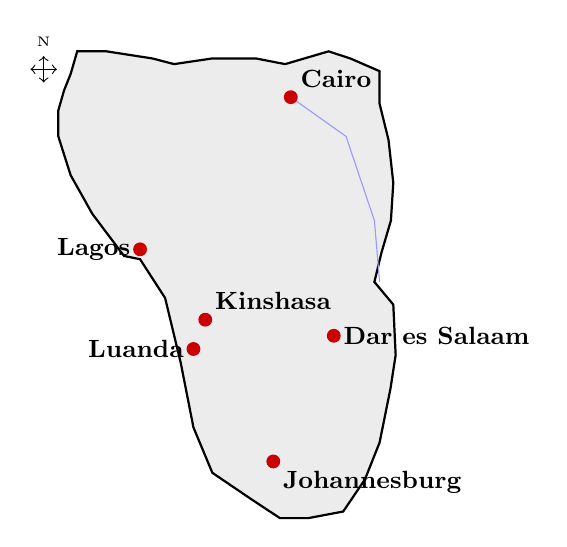
\begin{tikzpicture}[x=1cm, y=1cm, scale=0.6,]
 % ---- Africa outline (simplified polygon) --------------------
  % Points traced roughly clockwise from Morocco/NW corner.
  % Coordinates are (x,y) in the projection above.
  \draw[thick, fill=gray!15] 
    % NW: Morocco/Western Sahara coast, then across North Africa
    (0.97, 9.40)  % Cape Spartel ~35.8N, 5.9W
    -- (1.11, 9.88) % Strait of Gibraltar area ~37N, 5W (slightly in)
    -- (1.73, 9.88) % ~37N, 10E (Tunisia/Algeria north)
    -- (2.70, 9.73) % ~36N, 10E Tunisia
    -- (3.16, 9.61) % ~35N, 11E
    -- (3.97, 9.73) % ~36N, 12E Libya
    -- (4.89, 9.73) % ~36N, 17E
    -- (5.51, 9.61) % ~35N, 20E Libya
    -- (6.43, 9.88) % ~37N, 25E (Crete area, just clip)
    -- (6.89, 9.73) % ~36N, 28E
    -- (7.51, 9.46) % ~34N, 31E Egypt north (Nile delta)
    -- (7.51, 8.77) % ~30N, 31E  (Cairo latitude)
    -- (7.70, 8.00) % ~27N, 33E Red Sea coast
    -- (7.80, 7.10) % ~22N, 34E
    -- (7.75, 6.30) % ~18N, 33E Sudan/Eritrea
    -- (7.55, 5.62) % ~14N, 32E (Horn direction)
    -- (7.40, 5.00) % ~11N, 31E Djibouti area
    -- (7.80, 4.52) % ~8N,  34E Ethiopia/Somalia horn
    -- (7.85, 3.45) % ~2N,  34E Kenya east
    -- (7.74, 2.74) % ~1S,  32E
    -- (7.51, 1.60) % ~10S, 31E Tanzania
    -- (7.20, 0.82) % ~17S, 30E Mozambique
    -- (6.74, 0.14) % ~24S, 27E
    -- (6.00, 0.00) % ~35S, 21E Cape area west
    -- (5.40, 0.00) % ~35S, 16E
    -- (4.78, 0.41) % ~30S, 11E Namibia
    -- (3.97, 0.96) % ~25S,  4E ... Namibia/Angola
    -- (3.57, 1.92) % ~18S,  2W Angola coast
    -- (3.30, 3.29) % ~10S, -1W Angola/Congo coast
    -- (2.97, 4.66) % ~0,   -2W Gabon
    -- (2.44, 5.48) % ~6N,  -5W Ivory Coast/Ghana
    -- (2.10, 5.55) % ~7N,  -8W Liberia
    -- (1.43, 6.44) % ~14N,-13W Guinea/Senegal
    -- (0.97, 7.26) % ~20N,-16W Mauritania
    -- (0.71, 8.08) % ~27N,-18W W. Sahara
    -- (0.71, 8.63) % ~31N,-18W
    -- (0.83, 9.05) % ~33N,-17W Morocco
    -- (0.97, 9.40) % back to start
  ;



  % ---- Nile suggested with thin line --------------------------
  \draw[blue!40, thin]
    (5.63, 8.91) -- (6.80, 8.08) -- (7.40, 6.30) -- (7.51, 5.00);

  % ---- City dots ----------------------------------------------
  \tikzstyle{city}=[circle, fill=red!80!black, inner sep=0pt,
                    minimum size=5pt]

  \node[city] (cairo)    at (5.63, 8.91) {};
  \node[city] (lagos)    at (2.44, 5.69) {};
  \node[city] (kinshasa) at (3.82, 4.20) {};
  \node[city] (luanda)   at (3.57, 3.58) {};
  \node[city] (dares)    at (6.54, 3.86) {};
  \node[city] (jhb)      at (5.26, 1.20) {};

  % ---- Labels (positioned to avoid overlap) ------------------
  \node[above right, font=\small\bfseries] at (cairo)    {Cairo};
  \node[left,        font=\small\bfseries] at (lagos)    {Lagos};
  \node[above right, font=\small\bfseries] at (kinshasa) {Kinshasa};
  \node[left,        font=\small\bfseries] at (luanda)   {Luanda};
  \node[right,       font=\small\bfseries] at (dares)    {Dar es Salaam};
  \node[below right, font=\small\bfseries] at (jhb)      {Johannesburg};

  % ---- Compass rose (simple) ----------------------------------
  \begin{scope}[shift={(0.4,9.5)}, scale=0.35]
    \draw[->] (0,0) -- (0, 0.8) node[above, font=\tiny]{N};
    \draw[->] (0,0) -- (0,-0.8);
    \draw[->] (0,0) -- ( 0.8,0);
    \draw[->] (0,0) -- (-0.8,0);
  \end{scope}

\end{tikzpicture}
\end{adjustbox}

\be
\item Use the Sorted Edges algorithm to find a Hamiltonian circuit. List the cities of your circuit in order, starting and ending at Cairo.

\vspace{1.2in}

\item What is the total distance of your circuit? \ans

\item Nearest Neighbor starting at Johannesburg gave a tour of 17{,}870 km. How does your Sorted Edges tour compare? %Did you get the same circuit as Nearest Neighbor starting at Cairo?
\vfill
\ee

%\item Nearest Neighbor builds one path that grows from the starting vertex. How does the Sorted Edges algorithm build its circuit differently? Describe what the chosen edges look like partway through the algorithm.
%\vfill

\item The Sorted Edges algorithm can't always find the Hamiltonian circuit with the smallest weight. Explain why, and construct a small example where it breaks.
\vfill

\vfill

\vfill

\end{enumerate}
\end{document}
